\documentclass[11pt,a4paper]{report}
\usepackage[utf8]{inputenc}
\usepackage{csquotes}
\usepackage[myheadings]{fullpage}
\usepackage{blindtext}
\usepackage{enumitem} % Include this in your preamble

% Package for headers 
\usepackage{fancyhdr}
\usepackage{lastpage}

% For figures and stuff
\usepackage{graphicx, wrapfig, subcaption, setspace, booktabs}
\usepackage[T1]{fontenc}

% Change for different font sizes and families
\usepackage[font=small, labelfont=bf]{caption}
\usepackage{fourier}
\usepackage[protrusion=true, expansion=true]{microtype}

% Maths
\usepackage{amsmath,amssymb}
\usepackage{float}
\usepackage{graphicx}
\usepackage{wrapfig}
\usepackage[colorinlistoftodos]{todonotes}
\usepackage[colorlinks=true, allcolors=blue]{hyperref}

% Bibliography
\usepackage{biblatex} 
\addbibresource{references.bib}

%% Language and font encodings
\usepackage[english]{babel}

% Links and references
\usepackage{hyperref}

\newcommand{\HRule}[1]{\rule{\linewidth}{#1}}
\onehalfspacing
\setcounter{tocdepth}{5}
\setcounter{secnumdepth}{5}

%% Sets page size and margins
\usepackage[a4paper,top=2cm,bottom=1.5cm,left=1.5cm,right=1.5cm,marginparwidth=1.5cm]{geometry}

\pagestyle{fancy}
\fancyhf{}

% Header and footer information
\setlength\headheight{15pt}
\fancyhead[L]{MIS - 2023/2024} 
\fancyhead[R]{I.Re Depaolini, M.Carraro, T.Ceccherini, I.Rocchi}
\fancyfoot[R]{\thepage}
\makeindex

% This is a template for the essay. Do not change anything in this file except the title, author and date.
\begin{document}

\date{}

% Do not change anything here except in \LARGE \textbf{This is the title of the essay} 
% /hline before and after the title makes those horizontal lines appear, you can change the appearance by changing the 2pt to different sizes
\title{ \normalsize TRENTO UNIVERSITY
		\\ [1.0cm]
		% Change to your faculty if needed
		
\includegraphics[width=30mm]{img/unitn_logo.jpg}\\[.5cm]
		Faculty of Cognitive Science and Computer Science\\
		\textsc{Multisensory interactive system}\\[2.0cm]
		\LARGE \textbf{Enhanced rock paper scissors game with a multisensory interactive system}\\[1.5cm]
		\normalsize \today \vspace*{5\baselineskip}}


		
\date{}

\author{
  Icaro, Re Depaolini\\
  \texttt{icaro.redepaolini@studenti.unitn.it}
  \and
  Marco, Carraro \\
  \texttt{marco.carraro-1@studenti.unitn.it}
  \and
  Tommaso, Ceccherini\\
  \texttt{tommaso.ceccherini@studenti.unitn.it}
  \and
  Ilaria, Rocchi\\
  \texttt{ilaria.rocchi@studenti.unitn.it}
}


		 
\maketitle

% Uncomment the next line if you want a table of contents 
% \tableofcontents

\newpage


% Uncomment the next line if you want keywords/index terms after the abstract. 
%\textit{\textbf{Keywords}: lorem, ipsum, dolor}


\section*{Abstract}

This project explores the impact of multisensory feedback in enhancing the traditional game of Rock-Paper-Scissors through a newly developed interactive system. Our primary objective was to determine the role of vision in influencing the game's outcome by comparing player performance in blindfolded versus non-blindfolded conditions. The system integrates haptic feedback, auditory cues, and infrared distance sensors to provide a comprehensive multisensory experience.
Our findings suggest that the inclusion of multisensory feedback does not significantly impact the game's outcome, challenging the presumed dominance of visual information in player success. This offers a blend of technology and sensory integration, hence promoting accessibility and inclusivity in gaming.

\section*{Introduction}
Our project concerns the creation of a multisensory interaction system based on the classic game of Rock-paper-scissors, which is contextualized within an environment where the user receives feedback and stimulation through different sensory channels. The aim of the system is to observe whether vision plays a significant role in the ratio of victories of a player in the game Rock-paper-scissors. In order to achieve the aforementioned research goal, each pair of players perform the game in both of its versions: blindfolded and not-blindfolded. 
The created system provides the users discrete interactions (e.g. haptic feedback as a sensory response to the game result) as well as continuous interactions (e.g. infrared distance sensors used to set the game to a \texttt{“ready" state}).
The area of research involved in this project has potential applications in different fields, such as entertainment, accessibility, and sociality.
Our approach is based on some of the theoretical perspectives on multisensory perception and interactive systems introduced in the course.
For example, the concept of multisensory perception became apparent: we were able to observe how the senses do not operate in isolation, but combine with each other to create a unified perception of reality.
Through the feedback obtained from the users involved, moreover, it was interesting to recognize how their perception of the game and their activities performed varied within the two different modalities, also provoking different reactions and influencing their moods and level of involvement.
In this report, we will describe our project in detail, illustrating the design, technical implementation and evaluation of our system.

\section*{Related Work}

From the literature we have found few resources regarding the role of vision in games such as Rock paper scissors, however an interesting study has examined the impact of the mirror neuron system on player actions in Rock-Paper-Scissors, focusing on imitation's role in predicting game outcomes and the influence of autism spectrum traits on imitation abilities. It concluded that neither winning nor losing patterns were significantly affected by imitation, and there was no correlation found between participants' autism spectrum scores and their imitation levels, suggesting a minimal effect of the mirror neuron system in this competitive setting \cite*{4}.
One notable project is an auditory card game system designed to be accessible to visually impaired players by presenting card contents with auditory stimuli. This system aims to allow for equitable play among visually impaired and sighted players, focusing on the auditory experience as a primary interaction mode. The effectiveness of this system was validated through experiments, highlighting the potential for designing accessible board games that do not rely on visual information \cite*{3} .
Another related research explores strategies adopted by users with visual impairments in approaching, and sometimes completing, video games that don't offer accessibility settings. These strategies show potential new ways for designing games to be accessible while maintaining the core gameplay experience. It is interesting to notice that many of the strategies described in the paper are focused on finding ways to provide additional audible information to the player \cite*{5}.

\section*{Architecture and Design}
\begin{figure}[htbp]
  \centering
  \includegraphics[width=\textwidth]{img/design_system.png}
  \caption{Caption of the image}
  \label{fig:image_label}
\end{figure}

\noindent Our system is composed of several parts and components.
All of these components and their communication with other parts are explained in detail in their own section below \hyperref[sec:Implementation]{Implementation}.
The schematic architecture of our interactive system involves multiple components and two players. it is designed to create an immersive experience, for a game or simulation, utilizing various types of feedback and sensors. Here's a breakdown of the components and the communication between them:

\begin{description}
  \item [Node Server:] This is the central processing unit that handle network communication (UDP), runs on Express.js (a web application framework for Node.js), and includes functionalities such as CSV logging. 
  \item [Visual Monitor:] A display screen shows the visual output, used during the our pilot test phase, which is a 3D simulation of the hand. It is connected to the Node Server, receiving data to display the last move or action taken by the players.
  \item [PureData Patches:] PureData (Pd) is a visual programming language for creating interactive computer music and multimedia works. These patches are made to produce audio cues for the game and create audio effects that are triggered by certain actions in the system, for example, the sound produced by the interaction with IR sensors.
  \item [Sound Card:] It is an audio interface that processes the sound output from the PureData patches and sends the audio to the speakers.
  \item [Sound Speakers:] Represented by two JBL speakers, these output the audio for the players to hear, adding to the immersive experience.
  \item [Teensy Board:] A micro-controller board (similar to Arduino) programmed with Arduino code. It processes input from gloves and IR sensors and communicates with PD patches.
  \item [Gloves with Flex and Haptic Sensors:] These are worn by the players (Player 1 and Player 2) and are used to detect the movements and gestures of their hands. The flex sensors detect bending motions, while haptic sensors provide feedback to the user, through vibrations.
  \item [IR Sensors:] Infrared sensors are used to start a new round, the player has to place one hand on them and an audio feedback guide him by saying \texttt{“player one/two ready”}. These IR sensors are very useful in the blind version of the game, since they help the player in a navigation and detection process by tracking the hand position over the sensor.
  \item [Player 1 and Player 2:] Two participants in the system, each equipped with gloves that have sensors. They interact with the system and with each other within the context of the game or simulation.
\end{description}

\subsection*{Communication between components}
The communication between the components is essential for the system to work as intended. Here's a brief overview of how the components interact with each other:
\begin{itemize}
  \item The players make movements with their sensor-equipped gloves.
  \item The information about the “readiness” of the player are sent by PD to arduino
  \item The players play their rounds
  \item The Teensy Board processes these movements and sends the data to PD.
  \item Simultaneously there are trigger audio responses via PureData patches, which are then processed by the Sound-card and played through the Sound Speakers.
  \item PD sends the detected moves to the Node Server using an UDP connection and the [netsend] object in the main patch.
  \item The Node server receives the moves and saves all the rounds in a CSV file.
  \item The Node Server could also send commands to the Visual Monitor to update the display based on the players' actions exposing an Express endpoint called \texttt{‘/last-move’}.
\end{itemize}

\noindent All these components work together to create an interactive and immersive experience, with visual, auditory, and tactile feedback loops.
Our system is mainly designed to be placed on a stationary like a table or even on a couch , and not in a too noisy place, since the speakers provide cues about the game and the external noise could lead to a misunderstanding, increasing ambiguity among different moves and sounds.
We have developed this system with a focus on accessibility problems, trying to think how such a system could be used by vision impaired people without a big effort.
For example the increasing and decreasing sound that comes from the IR sensors detection, is designed to help the navigation and the placement of the users hands.
Moreover the integration of multiple feedback, using both audio cues and haptic ones, could also be useful for people with multiple disabilities \cite*{2}.
The main idea is to have a system that can guide the users in their games, and provide them the results and feedback of their moves in a comprehensive way.

\subsection*{Usage model}
In the current version, our system is primarily designed for research purposes. During the tests, the assistance of a researcher and an initial explanation of how the system works were necessary for the users. Despite that, the system is easy to use and takes a few minutes to become familiar with. This ease of use was also expressed by the users themselves in the System Usability Scale, the results of which are presented in more detail in the \hyperref[sec:Evaluation]{Evaluation section}.
When positioned in front of the system, the user can wear the glove and start to interact with the IR sensor while waiting for the opponent to wear the glove as well. When both players are facing each other, positioning the elbow at the suggested point on the table and with the hands wearing the gloves close to each other, they can both use their free hand to reach their own IR sensor and keep it there for two seconds to start the match. The sound \texttt{“player one”} will be played from player one’s speaker after the hand is detected for two seconds. The same will happen for the sound \texttt{“player two”}, playing from player two’s speaker. After both sounds have been played, the countdown sounds will be played from both speakers. At the sound of \texttt{“GO\!”}, players are supposed to play their moves and keep the hand still for a few milliseconds so that the move can be recorded by the system. The sounds corresponding to the moves are played: first, player one’s move will be heard, starting from speaker one; then, after a second, player two’s move sound will be heard starting from speaker two. We add this delay to avoid the precedence effect \cite*{1}. At this point, the players have understood who won the match, even if playing blindfolded, based on the heard sounds. The system will declare the winner playing a sound \texttt{“player one\/two wins”} from the winner’s speaker, then the game loop will start from the beginning, and the system will wait for players to be ready, placing their free hand on the IR sensors again.
Users can approach the system in different ways, using it for research purposes, playing the game of Rock-Paper-Scissors in a controlled environment, or simply challenging friends to a best-of-five game or a long series of matches.

\section*{Implementation}\phantomsection\label{sec:Implementation}

\subsection*{Teensy code}
The sketch on which the project consists of a main loop that corresponds to a single round of Rock-Paper-Scissors.
Within this main structure, four while loops were inserted to verify the time coordination between the code and Pure Data. With each loop, in fact, the arrival of a particular message from Pure Data on the serial port is verified, remaining pending until it is correctly received. In addition, there is a fifth while loop responsible for obtaining and subsequently mapping the data from the sensors into the relevant performed moves.
For any communication between the code and Pure Data, we used the \texttt{receive\_message} and \texttt{handle\_received\_message} functions. The first function is in charge of checking for new messages from Pure Data and, if positive, passes that information to the second function.
\texttt{Handle\_received\_message}, after handling the incoming data, verifies its content. Based on this we modify the global variables of our program, which allow the exit from the various while loops and the continuation of the main block.
At the end of the last while loop, the program sets the previously modified global variables back to their initial state, allowing users to start a new round.
\subsection*{Players ready}
The first block verifies that both players enter \texttt{"ready"} mode, that is, they are both ready to play. This check is done by continuously reading the values recorded by the IR sensors, with them being sent to Pure Data. Once a predetermined threshold has been passed, and the corresponding audio feedback has been received, Pure Data will send the \texttt{"players\_ready"} message, which will allow them to exit the loop and move on to the next step.
\subsection*{Countdown finished}
This second block was inserted for the purpose of activating the flex sensor reading only once the countdown is over. Pure Data, in fact, will communicate the end of this event through the \texttt{"countdown\_finished"} message. From here, the code will start the functions in charge of reading and mapping the moves performed by the users.
\subsection*{Reading flex sensors}
This while loop is the only one that does not require communication with Pure Data. In fact, its function is to verify the values obtained from the flex sensors, based of course on the movement performed by each user.
This is done through the \texttt{"checkFingers"} function which, after mapping each value to the corresponding PIN, collects the final values of each and passes them to the \texttt{"check\_move"} functions. For technical reasons, we had to create two separate functions, one for each hand, setting different threshold values that would signal each finger as \texttt{"open"} or \texttt{"closed"}. Based on the values returned by each finger, \texttt{check\_move} maps the move performed and returns an integer value, corresponding to the move recorded for each user. The two values are saved in the moves vector, which contains the moves of both players.

\subsection*{Sending moves and receiving response}
These two steps communicate the moves made by each user to Pure Data, which will take charge of returning the corresponding feedback to both, as well as acknowledging receipt of the moves, allowing the code to move to the next step.

\subsection*{Checking winner and giving haptic feedback}
With the confirmation of receipt of moves from Pure Data, the winner is verified through the classic Rock-Paper-Scissors rule of play and, unless there is no winner due to an invalid round, the number of rounds played is increased and the identity of the winner is communicated to Pure Data.
At this stage, the code, through the \texttt{"giveFeedback"} function, returns the respective haptic feedback to the users, divided into the various win/tie/defeat cases (the null round will cause the same feedback as the tie case).
\subsection*{Winner announced}
The last block verifies that Pure Data has received the information about the winner and has returned the relevant audio feedback. At the end of this the various global variables modified earlier are reset to their initial values, and the main loop can begin again for the next round.

\subsection*{Pure Data}

The Rock-Paper-Scissors matches were handled through the Pure Data code. The game starts if Teensy is connected to the laptop with the sketch \texttt{teensy\_control.ino} uploaded. The patch \texttt{[MAIN]} is initiated, and the right port for Teensy-Pure Data communication is assigned on Pure Data in the patch \texttt{[\_receive\_from\_Teensy]}. The same patch handles all the data channels used to receive and send information from and to Teensy. The match loops are organized through four patches that handle different phases of the game: \texttt{[\_IR\_wait]}, \texttt{[\_countdown]}, \texttt{[\_receive\_signs]}, \texttt{[\_declare\_winner]}. DSP is enabled and disabled every time a patch is accessed and left during the game loop. All the patches are initiated from the patch \texttt{[MAIN]}, where, at every step, we also send a message to Teensy to synchronize the game and the sensors' activation.

\subsection*{\textbf{[\_receive\_from\_Teensy]}}

Here, Pure Data receives data from Teensy and sends it to the patch where it is necessary. The data from IR sensors are received on channels \texttt{a0} and \texttt{a1}, and from a range that goes from 0 to 500, they are scaled to values between 0 and 5. Then, they are sent to the patch \texttt{[\_IR\_wait]}. Players' moves are mapped from the flex sensors and assigned to a value on the Teensy code (0 for rock, 1 for paper, 2 for scissors, 3 for an invalid move). These values are then sent to Pure Data through channels \texttt{d0} and \texttt{d1}. The result of the game is also calculated in the Teensy code and sent to Pure Data through channel \texttt{w0} (0 if a move was invalid, 1 if player one wins, 2 if player two wins, 3 if they drew). A channel called \texttt{fingers} was used to receive and print flex sensor values and detect which one was causing problems during debug phases.
\subsection*{\textbf{[\_IR\_wait]}}

This patch receives the scaled values of the IR sensors from the patch 
\texttt{[\_receive\_from\_Teensy]}
and uses them to detect when the player's hand is placed over the IR sensor. While the player's hand is detected, by moving it nearer or further from the IR sensor, it is possible to modulate the sound emitted. For player one the carrier and the modulator are phasor objects, while for player two they are oscillator objects. These two modulated sounds are sent, respectively, to \texttt{ch1} or \texttt{ch2} buffers that are connected to the Digital to Analog Converter object. When the hand is detected for more than 2 seconds, the audio signal stops, and instead, a sound saying \texttt{“player one”} or \texttt{“player two”} is sent to the DAC. Once both players' hands have been detected, the patch sends a bang to the following one in the game loop, also disabling DSP in the patch.

\subsection*{\textbf{[\_countdown]}}
This patch simply sends to both DAC channels four audio files that say, in order: \texttt{“three”, “two”, “one”, “GO!”}. On the last signal players are supposed to be playing their moves. The patch sends a bang to the following one in the loop, also disabling DSP.

\subsection*{\textbf{[\_receive\_signs]}}

Receives the moves played by both players from channels d0 and d1 and sends audio signals to the corresponding DAC channel. Player two's move is announced with a one-second delay compared to player one's move to reduce the ambiguity in hearing the two sounds at the same time and avoid the precedence effect \cite*{1}. When the signs played are received, they are also sent to a local server through UDP messages. In the server, data is collected in a CSV file for further analysis.

\subsection*{\textbf{[\_declare\_winner]}}
The last patch of the loop receives the game result on channel \texttt{\_w0} and sends a corresponding audio signal to DAC channels. If one of the players wins, the audio feedback \texttt{“player one/player two wins”} is sent to only DAC channel \texttt{ch1} or channel \texttt{ch2}. If the result is a draw or an invalid move was detected, both speakers will play the audio saying “no contest.” At this point, the game ends, and the Pure Data patch \texttt{[MAIN]} starts the game loop again. Now the system is back in the patch \texttt{[\_IR\_wait]} waiting for both players to be ready, listening to the IR sensors.
\subsection*{Wiring and system structure}

The physical components of the system include two gloves, two infrared proximity sensors, and a Teensy micro-controller, to which the aforementioned components are connected. Each glove is designed to track the movements of the players and provide haptic feedback in response to the outcome of each game. The players' movements are mapped using flex sensors (one on each finger), and vibrations are generated by coin vibration motors based on the game's result.
Considering the audio feedback provided as a response to the same events, such haptic response allows for a redundancy of information. Such overlap leads to the system being more robust and to the users' experience being enhanced.

\subsection*{Haptic feedback}
In the event of victory, vibrations are delivered to the tip of the forefinger, while in case of loss, they are delivered to the wrist. 
If a tie occurs, both types of vibrations are delivered simultaneously.
The location of the coin motors has been chosen based on the distribution of mechanoreceptors in the hand. In particular, given the nature of the provided vibrations, what has been taken into consideration is the distribution of the Meissner and Pacinian corpuscles \cite*{6}. 
Consequently, the victory-related vibration response has been placed on the tip of the forefinger. The second motor has been placed considering the fact that spatial separation of haptic stimuli can enhance the clarity and distinction between them, hence enabling users to better interpret the haptic information provided. This led to the placement of the second motor on the wrist, which is a considerably different and distinguishable area of the glove. 
Moreover, \cite*{7} suggests that positioning actuators on the wrist might improve the effectiveness of conveying information through vibrotactile feedback. 

\subsection*{Flex sensors}
The flex sensors have been placed on each finger. In order to map the hand movements performed by the players, an analysis has been conducted to determine the proper thresholds that allow the system to determine if a finger is open or closed.

\subsection*{Teensy micro-controller}
All the mentioned physical components are connected to a Teensy micro-controller. Using a Teensy instead of an Arduino allows the usage of a greater number of analog and digital I/O options in comparison to the Arduino board. 

\subsection*{Visual Monitor}
This part of the system was used by the group just for a testing purpose. We have decide to include it in our system to better understand what could have been possible future developments.
The visual monitor folder consist in two distinct parts:
\begin{itemize}
  \item The client
  \item The server
\end{itemize}
\subsection*{Client}
The client component is a 3D web application leveraging technologies such as \href{https://threejs.org/}{Three.js} for rendering 3D graphics, \href{https://gsap.com/}{GSAP} for smooth animations. It designed to display and interact with a 3D model of a hand, capable of reflecting updates and movements fetched from the server.

\subsection*{Server}
On the flip side, the server component is built on Node.js and plays a pivotal role in managing communications between the client and Pure Data, alongside generating a CSV file for data logging and analysis. It acts as the backbone of the system, processing real-time game move data via UDP communication from PD and providing RESTful interfaces for the client to fetch the latest game moves.

\subsection*{Three.js for 3D Graphics}
The code begins with importing the necessary modules from Three.js, including the core library, \texttt{`OrbitControls`} for camera control, \texttt{`GLTFLoader`} for loading 3D models, and \texttt{`OutlineEffect`} for adding an outline effect to the 3D objects.
A new Three.js scene is created, and the background color is set based on predefined defaults. This is an essential step for setting up the environment in which the 3D model will be placed.
A GLTF model of a hand is loaded using \texttt{`GLTFLoader`}, and upon successful loading, it's added to the scene. Additionally, materials and bones of the model are set up to allow for interactive control and customization.

\subsection*{GSAP for Animation}
GSAP (GreenSock Animation Platform) is used to animate the properties of the hand model and the scene's colors dynamically based on the moves fetched from the server or user interactions.

\subsection*{Data Fetching}
A Proxy object is used to wrap the \texttt{`handsMove`} object, ensuring that any changes to the hand moves are intercepted and handled appropriately.
The application periodically fetches the latest move from a server and updates the \texttt{`handsMove`} object accordingly. This functionality suggests the hand model's movements could be synchronized with external data or controls.

\subsection*{Interactive 3D Model Control}
Functions \texttt{`setMaterials`} and \texttt{`setBones`} are defined and used to adjust the materials of the model and the rotation of bones, to simulate movements such as clenching or spreading fingers, respectively.
The application integrates animations with GUI controls, allowing users to dynamically control the model's appearance and pose with immediate visual feedback.
This part uses modern web technologies for 3D visualization and interaction. It showcases how Three.js can be combined with GSAP for animations, creating a highly interactive and customizable 3D application. 

\subsection*{Server and Node.js}
The Node.js server serves two main goals, the first one is handling the communication between PD and the Visual monitor client, the second one is to produce a CSV file, like a logging system, that we used for the data analysis. 
The application is designed to communicate with Pure Data using UDP for real-time game move data exchange, and to expose an Express server for the REST communication with the client.

\subsection*{Integration with Pure Data}
The UDP server set up in the Node.js application listens for messages on port 41234, which are sent from a Pure Data patch. This setup allows for real-time communication between the PD environment and the Node.js application. The PD patch is expected to send messages that represent game moves, encoded as integers, for two players \texttt{(p1 and p2)}.

\subsection*{Game Logic Interaction}
Upon receiving a message from PD, the Node.js application processes it by extracting the player identifier \texttt{(p1 and p2)} and the move they've made. This is done within the `handleMessages` function, which updates an array `moves` that tracks the latest moves from both players.

\subsection*{Game State Logging}
The application not only processes these moves in real-time but also logs them to a CSV file \texttt{`games.csv`} after every two messages (representing a complete game round). This log includes timestamps, the moves made by both players in a human-readable format, and the winner of each round, as determined by the \texttt{`declareWinner`} function.

\subsection*{Hands Feedback to Clients}
The Express server's \texttt{`\/last-moves`} endpoint allows clients (which could be web interfaces, other applications) to fetch the latest game state. This enables a form of real-time feedback loop where the outcome of interactions in the PD environment can be reflected in other platforms or visualizations.

\section*{Evaluation}\phantomsection\label{sec:Evaluation}
The system we described in the previous section was used by the research group to test and validate the following hypotheses:
\begin{itemize}
  \item [\textbf{h0:}] Using our interactive system vision doesn’t have a significant impact on the ratio of victories of a player in the game Rock-Paper-Scissors.
  \item [\textbf{h1:}] Using our interactive system vision has a significant impact on the ratio of victories of a player in the game Rock-Paper-Scissors
\end{itemize}

\noindent Other than these hypotheses, the tests were also aiming at evaluating the system and participants feelings towards the experience of using it.
We selected participants among students of university of Trento, in particular, students living in Sanba student housing. We have excluded from the research people not being familiar with the game. By applying this selection, we made sure that all the people using the system had similar demographic characteristics and their performances in the game are less likely to be influenced by age or cognitive capabilities differences among participants. 

\noindent We performed two user test sessions in different shared rooms of Sanba student housing. The system was placed on a table of these rooms and participants were chosen randomly, in pairs, among students in the study rooms of the dormitory or that were found walking by the area where we were doing the tests. When approached, they were introduced to the research we were conducting and asked if they were familiar with the game Rock-Paper-Scissors. If so, the pair of students was asked to sit at the system, wear the gloves, and start playing three trial matches to become familiar with the game functions, the audio and haptic cues corresponding to each sign and to learn how to use the IR sensors to start a match. After the trial matches, the players were asked to play more or less 12 matches blindfolded and then the same amount of matches not blindfolded. For every pair of participants we switched which game mode would have been played first. At the end of the series of matches, participants were asked to answer a questionnaire and give feedback on the system quality, then they were asked to participate in a quick double interview where they were asked to discuss and elaborate on some aspects related to the system itself and the experience.

\subsection*{Results analysis}
During the testing phase, we have collected the users data regarding the winning percentages, with a csv file, created by the node server while the player were using the system.
Using a python script we have created a dataframe using \href{https://pandas.pydata.org/docs/index.html}{pandas} that we have analyzed and using the statistic library \href{https://www.scipy.org/}{scipy}.

\noindent Before performing any hypothesis tests, we have assessed the distribution of the data.
Firstly By examining the graphical distribution of the winning percentages for both the non-blind and blind modes, and then using the Shapiro-Wilk test.
\noindent The histograms in Figure \ref{fig:win_rates} show that the winning percentages for both the non-blind and blind modes are approximately normally distributed. 
This is further supported by the Shapiro-Wilk test for normality, which yields p-values of approximately 0.073 and 0.091 for the non-blind and blind mode winning percentages, respectively.
Additionally, the Q-Q plot in Figure \ref{fig:qq_plot} visually supports this finding. The data points closely follow the 45-degree line, indicating that the differences are approximately normally distributed.

\begin{figure}
  \begin{minipage}{0.5\textwidth}
    \centering
    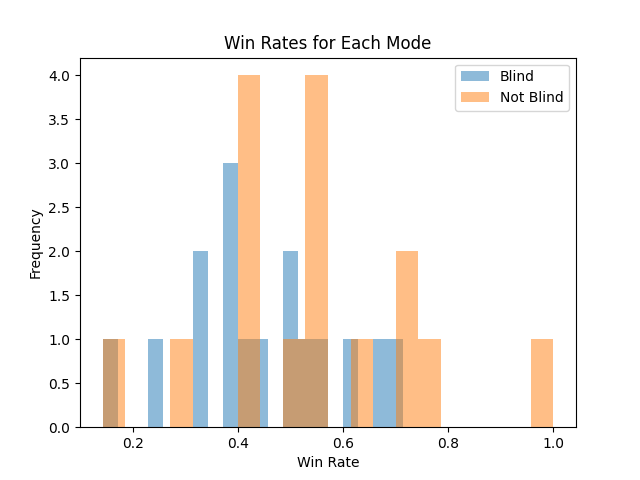
\includegraphics[width=\textwidth]{img/win_rates.png}
    \caption{Win rates blind-non blind Plot}
    \label{fig:win_rates}
  \end{minipage}%
  \begin{minipage}{0.5\textwidth}
    \centering
    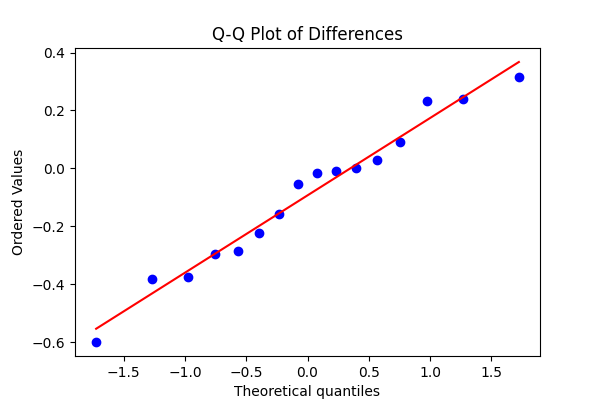
\includegraphics[width=\textwidth]{img/qq_plot.png}
    \caption{QQ plot}
    \label{fig:qq_plot}
  \end{minipage}
\end{figure}

\noindent Based on these results, it's reasonable to justifying the use of parametric tests like the paired samples t-test for analyzing these data.

\noindent Before starting the t-test we have normalized the data removing from the 32 players winnings, all the paired couples, in order to not have a dependence between the data.
Now that we've confirmed the normality of the data, and normalized the series, we have proceeded with the hypothesis test. We have used a paired samples t-test to compare the winning percentages between the non-blind and blind modes. The paired samples t-test is commonly used when there are two measurements on the same group, subject, or entity, taken under different conditions (for example, before and after a treatment, or in two different experimental conditions such as non-blind and blind modes in this context).
The results of the paired samples t-test have been used to compare the difference between two groups of data (in this case, the winning percentages in non-blind and blind modes) to see if this difference is statistically significant. 
The paired samples t-test between the non-blind and blind mode winning percentages resulted in a \textbf{t-statistic = -1.4700373650445964}, \textbf{p-value = 0.1622143698930308} .
A p-value greater than 0.05 (a common threshold for statistical significance) suggests that there is not enough evidence to reject the null hypothesis. In other words, there is no statistically significant difference between the winning percentages in non-blind and blind modes. This suggests that, on average, the mode of the game (non-blind vs. blind) does not significantly affect the winning percentages of the players in this sample.

\noindent This finding has important implications for game design and player experience. It suggests that the blind mode does not significantly disadvantage players in terms of winning percentages compared to the non-blind mode. This may help inform decisions about game design and accessibility, as it indicates that the blind mode does not significantly impact player performance in this context.

\subsection*{System evaluation}

\noindent The closed-ended questions included in the questionnaire were asked to evaluate the system according to the System Usability Scale. The system received an average score of 82.34 among the 32 participants who answered the questionnaire. Here the results of the SUS questionnaire: \href{https://github.com/icaro-rdp/enhaced-rock-paper-scissors/blob/main/Research/Quantitative/SUS/sus_results_breakdown.png}{SUS results}.
After answering the closed-ended questions, participants answered three more open-ended questions. A researcher facilitated the interview, recording the answers and collecting information from the participants about the system features and the impact that playing blindfolded had on the game. The interviews were transcribed and analyzed, together with observational notes taken during the tests. From those documents, several pieces of information about the game experience and participants' opinions about the system emerged. The observations were useful to analyze the user's interaction on a visceral level and identify if there were some parts of the interaction with the system that were not easy to understand.

\noindent It emerged that sometimes one of the players was uncertain, even after some matches, about which number was assigned to them. This suggests that audio cues could have been diversified more on the two speakers, or it should have been stated in a clearer way in the tutorial phase which player number was assigned to each participant. We also noticed that performing scissor symbols was sometimes troublesome for some players. In a few cases, the player was not closing the little finger and ring finger enough to allow the system to detect the move. We observed stronger reactions to draws and noticed that some participants were having trouble understanding how the IR sensor works. This was confirmed by the participants themselves during the interviews. These pieces of information, along with those from the interviews, were collected in a \href{https://github.com/icaro-rdp/enhaced-rock-paper-scissors/blob/main/Research/Qualitative/InterviewsAnalysis.png}{thematic graph} available in the GitHub repository of the project. 

\noindent The five thematic areas that emerged are: 
\begin{itemize}
  \item Liked features of the system
  \item Disliked features of the system
  \item Participants suggestions on how to improve the system
  \item Participants feelings
  \item Differences between the two game modes
\end{itemize}
\subsection*{Liked features of the system}
From the interviews and observations conducted during the tests, it emerged that participants enjoyed using the system. Particularly, some of the most liked features were the tactile vibration, defined as \texttt{“pleasant”}, and the sounds. The sounds were appreciated, both those corresponding to the game moves and those announcing game phases and the match result. Many participants associated the voices used for the countdown and announcing the result with voices used in vintage video games or sports announcers.
\begin{center}
  \textit{"Speaking of positive aspects, I find the tone of the speaker's voice very engaging—very American, like a sports game. I really like it."}
\end{center}

\subsection*{Disliked features of the system}
Among features that players criticize, first of all, it emerged that the IR sensors that players had to use to confirm they were ready for the match were found excessively complex, and the same functionality could have been implemented in an easier way, like through the use of a button or a specific hand gesture. It was defined as \texttt{“difficult to find”}, and the sound played while the hand is detected by the sensor has also been defined as \texttt{“annoying”} by a participant. The gloves' structure was also reported to be fragile, and many participants reported being worried about damaging them
\subsection*{Participants suggestions on how to improve the system
}
Given the list of liked and disliked features that emerged, several suggestions on how to improve the game were mentioned by the participants. For example, it was suggested to make the gloves work with wireless technology to make them easier to wear and simplify the structure. It was also suggested to, instead of simply playing blindfolded, implement visual effects using Virtual Reality goggles to enhance the game experience. To make the game flow smoother, a participant suggested adding an audio or tactile feedback reminding both players that they had to confirm they are ready to play again after each match.

\subsection*{Participants feelings}
Overall, most of the pairs showed positive behavior towards the experience, reporting having fun using the system, mentioning the feeling of novelty that playing a simple game like Rock-Paper-Scissors in such particular conditions gives them. They all seemed interested in the research we were conducting and reacted positively to the system feedback and audio cues.

\subsection*{Differences between the two game modes}
When asked about differences experienced in playing the two game modes, participants described the blindfolded version of the game as more interesting, easier, and fairer. For some players, this mode allows them to concentrate more on the other player's moves, not having other distractions that require their attention. This brought, in their opinion, better results in their matches. For some others, the only effect that playing blindfolded had on the matches was just a randomization of the results, not being able to collect any visual cues of which moves the opponent was going to play.

\section*{Discussion and Conclusion}
The evaluation of the Enhanced Rock-Paper-Scissors system yielded insightful findings on the role of vision and multisensory feedback in gameplay. Despite the integration of haptic and auditory feedback, our statistical analysis did not support a significant difference in the winning ratios between blindfolded and non-blindfolded play, might suggesting that multisensory feedback compensates effectively for the lack of visual cues. This outcome aligns with the concept of multisensory integration, where different sensory inputs can create a coherent perception, thus maintaining the competitive balance of the game.

\noindent The system was well-received, with participants appreciating the immersive experience provided by the tactile vibrations and auditory cues. However, challenges with the IR sensor's complexity and glove fragility highlighted areas for improvement. 

\noindent The limitations encountered, such as the difficulty in interpreting IR sensor data and the glove's fragility, have the potential to guide our future endeavors in this field.

\noindent The collaborative efforts of our team, from system design to user testing, have been pivotal in achieving the project's objectives. This project has not only contributed to our understanding of multisensory interactive systems but also opened avenues for future research in enhancing user experience through sensory integration.


\section*{Group members contribution}
\begin{itemize}
\item \textbf{Icaro:}
  \begin{itemize}[noitemsep]
  \item Visual monitoring of the hands
  \item Server for logging of the data and PD communication
  \item Research design (quantitative)
  \item Data analysis (SUS \& hypothesis testing)
  \item Testing the prototype with users
  \end{itemize}

\item \textbf{Ilaria:}
  \begin{itemize}[noitemsep]
  \item Researching the best solutions for glove making
  \item Physical realization of the glove
  \item Mainly responsible for physical connection between system parts (cables, glove, Teensy, board)
  \item Testing the prototype with users
  \end{itemize}

\item \textbf{Tommaso:}
  \begin{itemize}[noitemsep]
  \item Realization of the structure of Pure Data
  \item Communication Pure Data - Teensy
  \item Data analysis (SUS \& hypothesis testing)
  \item Testing the prototype with users
  \end{itemize}

\item \textbf{Marco:}
  \begin{itemize}[noitemsep]
  \item Writing the code for the Arduino/Teensy part
  \item Communication Teensy - Pure Data
  \item Collaboration in the physical realization of the glove
  \item Testing the prototype with users
  \end{itemize}
\end{itemize}

\section*{Code appendix}
All the code can be found in the public github repository here: \url{https://github.com/icaro-rdp/enhaced-rock-paper-scissors }


\printbibliography
\addcontentsline{toc}{section}{Bibliography}


\end{document}